\chapter{Risposte orale Chessa}

\section{Interoperabilità di reti IoT}

\begin{figure}[htbp]
   \centering
   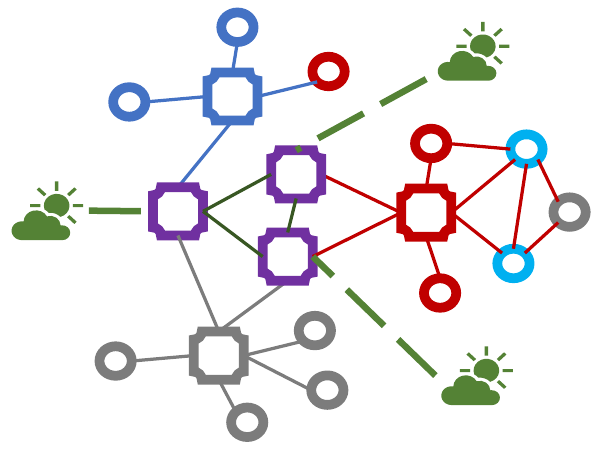
\includegraphics{images/questions/Schermata del 2023-10-19 10-03-17.png}
   % \caption{}
   \label{fig:dom1}
\end{figure}
Un problema comune nelle reti di device IoT sono i \textit{Vertical Silos}, business model adottato da diversi vendor, che porta le soluzioni IoT ad avere vari \textbf{vendor lock-in}, fra cui la limitatezza dei protocolli utilizzabili dai dispositivi prodotti.\\
Il problema è parzialmente risolto dagli \textbf{standard} di comunicazione, che tuttavia possono comunque essere ``troppi'' in una rete ampia, creando la necessità di tradurre da uno all'altro per permettere l'interoperabilità fra dispositivi di vendor diversi.\\
Primo argine al problema sono i \textbf{service gateway} (azzurro, rosso e grigio in figura), che permettono agli end-device di comunicare con internet (o altri gateway come in figura) e ad internet di comunicare con essi attraverso un endpoint unificato.\\
\ul{I dispositivi sono partizionati} \textit{non} in base al vendor, bensì \ul{al protocollo di comunicazione} che utilizzano.

Quella rappresentata in figura è una rete formata da \textbf{integration gateway} distribuiti che eseguono un mapping dai protocolli usati da end-device e service gateway (``non-viola'' in figura) a un linguaggio intermedio utilizzato per le comunicazioni fra di essi, e poi nuovamente mappato in un altro protocollo.
Questo permette di avere $2n$ mapping piuttosto che $n\times n$.
\note{Nella figura sembra che utilizzino lo stesso protocollo ``verde'' per comunicare con internet, ma non è necessario.}

All'interno di reti composte da device appartenenti a vendor (costruttori) diversi, che utilizzano protocolli diversi, è necessario l'utilizzo di un integration gateway per permettere l'interoperabilità tra i vari device.
%L'integration gateway quando non ha la capacità di tradurre un protocollo, traduce il comportamento di un device che utilizza un determinato protocollo in modo tale che device appartenenti ad altri vendor possano interagire con esso.
Mentre tradurre la serializzazione di un oggetto può essere vista come una funzione bigettiva/invertibile, per, ad esempio, richieste e risposte la traduzione da e verso il protocollo intermedio può richiedere operazioni differenti, da cui la necessità di $2n$ mapping, $\textit{n protocolli} \longrightarrow {lang\;intermedio}$ e viceversa.

\section{Sicurezza nei sistemi IoT}

\begin{figure}[htbp]
   \centering
   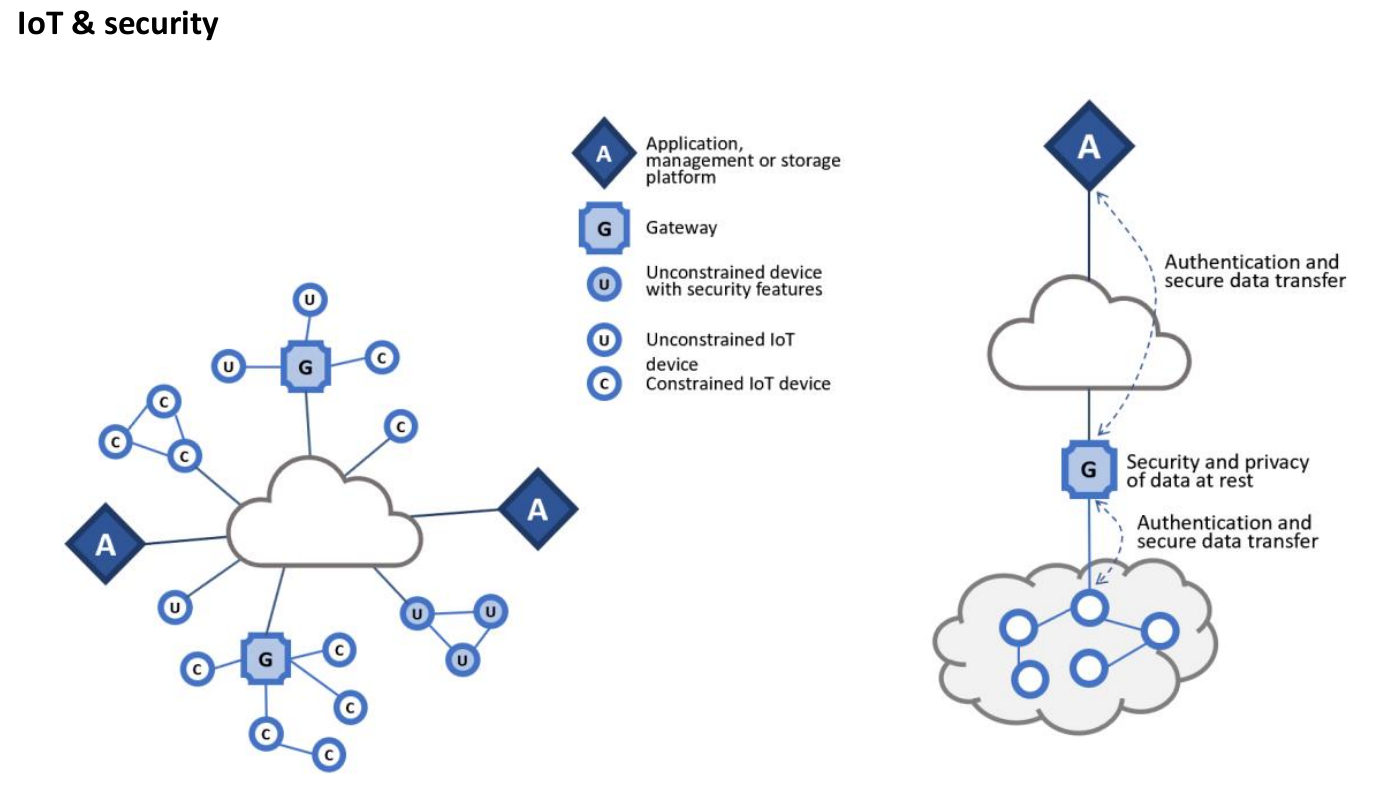
\includegraphics{images/questions/Schermata del 2023-10-16 18-20-38.png}
   % \caption{}
   \label{fig:dom2}
\end{figure}
Il tema della sicurezza in ambito IoT è un tema molto importante, in quanto per loro natura molte volte i dispositivi IoT sono sprovvisti di feature di sicurezza. Questo problema deriva dal fatto che i costruttori di questi device  danno priorità al time-to-market e al minimizzare il costo di produzione, a scapito della sicurezza:
le performance sono affette negativamente da essa, così come la durata della batteria. Spesso il sistema operativo installato è ``leggero'' e quindi privo di quelle funzionalità di security integrate all'interno di un sistema operativo full-fledged;
inoltre raramente vengono realizzate patch di sicurezza per i dispositivi IoT, e anche in tal caso è difficile applicarle. 

Per questo motivo sono stati standardizzati dall'ITU-T nel documento \texttt{Y.2066} dei \textit{requisiti di sicurezza} che riguardano diversi ambiti, tra i quali: comunicazioni, mutua autenticazione e autorizzazione, gestione dei dati, fornitura dei servizi, integrazione di politiche e tecniche di sicurezza e infine di security audit.
Tuttavia, non viene specificato come implementare soluzioni che soddisfino tali requirements.

Il focus dell'immagine è quello di mostrare quanto sia difficile garantire la sicurezza di una rete IoT, soprattutto in prossimità dei punti di accesso alla rete, questo dovuto anche al fatto che i dispositivi connessi sono di diversi tipi, esistono infatti dispositivi \emph{constrained} con limitate capacità computazionali e sprovvisti di ogni funzionalità di sicurezza, dispositivi \emph{uncostrained} con un'alta capacità computazionale ma senza funzionalità di sicurezza e altri dispositivi \emph{uncostrained} che però implementano funzionalità di sicurezza.\\
L'autenticazione mutua o one-way è fornita dai gateway. La sicurezza dei dati che si pone su tre livelli diversi: 

\begin{enumerate}
\item i dati salvati nei gateway e sui dispositivi;
\item i dati trasferiti tra gateway e dispositivi;
\item i dati trasferiti tra gateway e applicazioni.
\end{enumerate}

Tali requisiti di sicurezza diventano però difficili da soddisfare quando parliamo di constrained device, i quali raramente possono gestire encryption e autenticazione, portando a problemi di privacy sui dati, soprattutto riguardo i dispositivi nelle case.
È il caso dei dispositivi ``c'' in figura esposti direttamente a internet. 
\note{Possibile esempio climatizzazione, luci, frigo ecc\dots Oppure wristband e heart rate}

\section{Publish/subscribe e MQTT}

\begin{figure}[htbp]
   \centering
   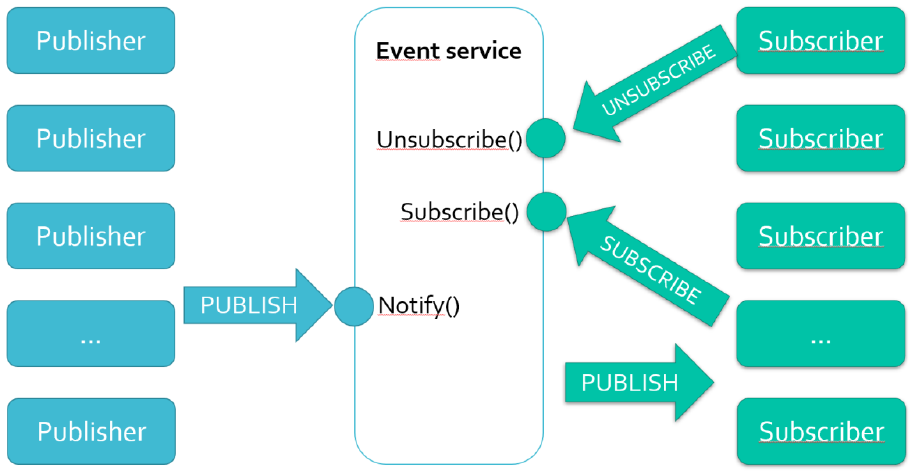
\includegraphics{images/questions/Schermata del 2023-10-19 12-23-59.png}
   % \caption{}
   \label{fig:dom3}
\end{figure}

MQTT è un protocollo di trasporto di messaggi affidabile e leggero basato sul modello publish/subscribe, un modello di comunicazione asincrona basato su eventi in cui sono coinvolte tre tipologie di entità: 

\begin{itemize}
\item il message broker, o event service: funziona come un server che gestisce lo scambio dei messaggi basato su topic;
\item i publisher: funzionano come client che pubblicano messaggi sul message broker marcandoli con un determinato topic;
\item i subscriber: funzionano come client e si sottoscrivono ad un determinato topic sul message broker.
\end{itemize}
\note{I client devono conoscere l'IP/hostname del broker \textit{beforehand}, essendo MQTT basato su TCP/IP.
I client sono identificati dal broker attraverso un \textit{Client ID} che deve essere univoco.}

Quando un publisher pubblica un nuovo messaggio su un topic il message broker invia una notifica a tutti i subscriber che sono iscritti a quel topic, se ne esistono. Ogni subscriber è libero di disiscriversi da un determinato topic in ogni momento.
\note{I subscriber potrebbero anche essere offline al momento del publish, ma comunque ricevere successivamente il messaggio (se e solo se i messaggi hanno QoS 1 e 2) in caso abbiano richiesto una sessione persistente;
i messaggi possono anche essere \textit{retained}, e in tal caso vengono inoltrati non appena un client si sottoscrive al topic di appartenenza.}

Questo modello permette la non dipendenza tra spazio, tempo e sincronizzazione facendo si che tutti gli agenti possano lavorare in modo indipendente senza dover attendere il lavoro di altri. La scalabilità è inoltre migliore rispetto a un generico client/server, in quanto basta aggiungere più broker che funzionano in paralleo.

Il broker può filtrare i messaggi basandosi su tipo, contenuto e \textit{topic}.

\section{MQTT esempio di interazione e QoS}

\begin{figure}[htbp]
   \centering
   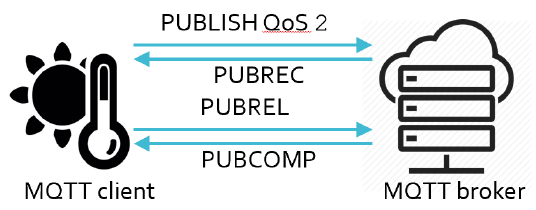
\includegraphics{images/questions/Schermata del 2023-10-19 15-29-05.png}
   % \caption{}
   \label{fig:dom4}
\end{figure}

Nell'immagine viene mostrato uno scambio di messaggi tra un client e il broker MQTT (event service) in cui nello specifico si nota il QoS 2 del pacchetto inviato. MQTT infatti offre una politica di QoS che risulta essere un accordo tra client e broker con 3 diversi livelli:

\begin{itemize}
\item Livello 0 (at most once): consegna best-effort senza garanzie, dove non abbiamo riscontri da parte del broker/server, il quale non salva i messaggi (neanche in caso di sessione persistente);
\item Livello 1 (at least once): consegna garantita almeno una volta al destinatario, dove il broker conferma la ricezione del messaggio tramite una risposta \texttt{PUBACK} (il messaggio può anche essere recapitato più volte);
il broker invia il messaggio ai subscriber subito. In caso \texttt{PUBACK} sia perso, il client invierà di nuovo il messaggio, e il broker potrà scartare il duplicato (non per forza), ma qualora avesse scartato il riferimento al messaggio (e.g. refresh cache), il messaggio duplicato verrà processato nuovamente e inviato ai subscriber.

\item Livello 2 (exactly once): garantisce la consegna esattamente una volta attraverso doppio two-way handshake, dove il broker notifica prima la ricezione del messaggio tramite un messaggio \texttt{PUBREC}, il client elimina il messaggio e risponde con \texttt{PUBREL} (\textit{``Release''}), il broker scarta il riferimento al messaggio e lo invia ai subscriber, infine termina lo scambio con \texttt{PUBCOMP} (\textit{``Complete''}).
\end{itemize}

\note{Solo \texttt{PUBREC} non risulta essere sufficiente, dato che se perso, il client manderà di nuovo un messaggio, quindi il broker deve salvare un riferimento del messaggio, che verrà scartato quando otterrà \texttt{PUBREL}.}
\section{MQTT}

\begin{enumerate}
\item \textit{Explain how messages are filtered by the broker and what are the topics in MQTT:} I messaggi vengono filtrati dal broker basandosi su tre diverse caratteristiche: il topic del soggetto (cioè l'argomento di interesse che tipicamente è una stringa), il contenuto (cioè una specifica query che controlla uno o più dati) oppure sul tipo (cioè controllando sia il contenuto che la struttura riferendosi ad una classe/tipo di dati). 

I topic sono stringhe organizzate in una gerarchia (ognuna separata da "/") che permettono di identificare un argomento di interesse. 
I subscriber possono utilizzare le wildcards per specificare un gruppo di topics:
\begin{itemize}
   \item \texttt{home/firstfloor/\textred{+}/presence}\\
   Seleziona tutti i \texttt{presence} sensors in tutte le stanze di \texttt{firstfloor}.
   Il \textred{+} è una wildcard che seleziona un solo livello della gerarchia.
   \item \texttt{home/firstfloor/\textred{\#}}\\
   Seleziona tutti i sensori del primo piano.
   Il \textred{\#} è una wildcard che seleziona tutti i rimanenti livelli della gerarchia, deve essere l'ultimo carattere del topic.
   \item I topic che iniziano con il carattere ``\texttt{\textred{\$}}'' sono riservati per statistiche interne di MQTT;
   Questi topic non sono standardizzati, e non possono essere pubblicati dai client.
\end{itemize}

\note{Notare che isciversi a \texttt{/home/firstfloor}, \textbf{non} significa ricevere notifiche per i messaggi relativi a tutti i subtopic come \texttt{/home/firstfloor/presence}, è necessario usare l'opportuna wildcard multilivello \textred{\#}}


\item \textit{Explain the persistent sessions in MQTT:} Una sessione persistente mantiene lo stato tra il client e il broker, e.g. se un subscriber si disconnette, quando si connette nuovamente non ha bisogno di iscriversi ancora una volta ai topic a cui era sottoscritto. Le sessioni sono associate al \emph{clientId}. 
È necessario richiedere la sessione persistente al momento della connessione, settando a \texttt{FALSE} il flag \texttt{Clean Session}.\\
Il broker memorizza tutte le iscrizioni, tutti i messaggi con QoS 1 e 2 non ancora confermati e che arrivano quando il client è offline.
\note{Si ricorda che il \texttt{Client ID} deve essere univoco per evitare complicazioni.}

\item \textit{Explain the retained messages in MQTT}: I retained message sono messaggi utilizzati dai publisher che vogliono tenere aggiornati i nuovi subscriber sullo stato delle comunicazioni. Questi messaggi sono semplici messaggi con il \emph{retainFlag} settato a \textbf{true}, ciò permette al broker di salvare e poi recapitare il messaggio ad un nuovo client che si sottoscrive a quel determinato topic, anche se il messaggio ha QoS 0. Solitamente questa tipologia di messaggi viene utilizzata per aggiornamenti non frequenti dello stato, come ad esempio lo stato di apertura/chiusura di una porta.


\item \textit{Explain the Lastwill\&testament and the Keep Alive mechanism in MQTT:} Sono due meccanismi utilizzati in MQTT, e fanno riferimento agli omonimi campi nel messaggio \texttt{CONNECT}:
\begin{enumerate}
   \item \textbf{LastWill\&Testament} è una feature che viene impostata a tempo di connessione da un client per notificare gli altri client in caso di una sua disconnessione improvvisa. Quando il broker riscontrerà una disconnessione improvvisa del client invierà il messaggio indicato a tutti gli iscritti del topic specificato quando la feature è stata impostata.

   \item \textbf{KeepAlive}: assicura che un client rimanga attivo, per farlo il client invia periodicamente un messaggio \texttt{PINGREQ} (seguito da \texttt{PINGRESP}) al broker prima che l'intervallo definito nel campo. Se questo non avviene in tempo il broker termina la connessione ed invia il messaggio \textit{LastWill\&Testament} se presente.
\end{enumerate}
\end{enumerate}

\newpage
\section{Zigbee I}

\begin{figure}[htbp]
   \centering
   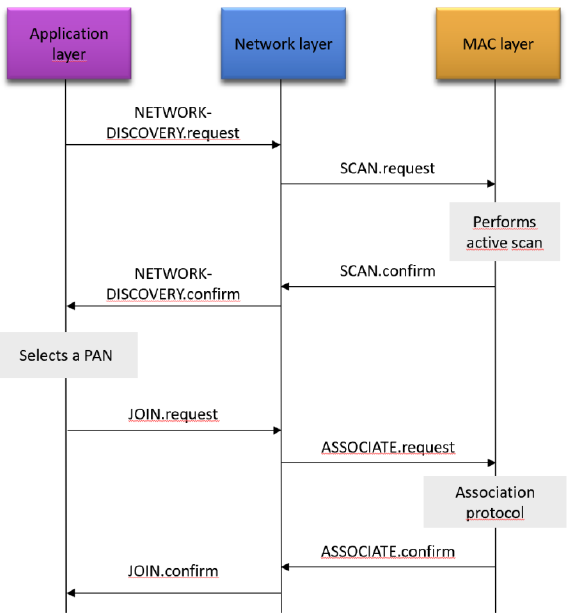
\includegraphics{images/questions/Schermata del 2023-10-19 15-30-53.png}
   % \caption{}
   \label{fig:dom6}
\end{figure}

Un device ZigBee può connettersi a una PAN in seguito a una richiesta specifica del Coordinator: in tal caso si tratta di \textbf{Direct Join}.
La figura invece illustra la procedura di \textbf{join through association} avviata da device ZigBee con un Coordinator di una PAN selezionata a seguito di una scansione preliminare.\\ 
I messaggi in sequenza sono:

\begin{enumerate}
\item La prima richiesta inviata è una \texttt{NETWORK-DISCOVERY.request}, che il livello applicativo manda al sottostante livello di rete per identificare le PAN disponibili;
\item Il livello di rete inoltra tale richiesta al livello MAC ---inviando una \texttt{SCAN.request}--- che avvia una active scan che restituisce al livello di rete una serie di PAN ID, con informazioni sui relativi router/coordinator, attraverso una \texttt{SCAN.confirm};
\item Il livello di rete propaga a livello applicazione il set di PAN ID con \texttt{NETWORK-DISCOVERY.confirm}, permettendo la selezione della PAN a cui unirsi;
\item La \texttt{JOIN.request}, che viene inoltrata al network layer, contiene dei parametri come \ul{l'identificatore della PAN scelta}, un flag che indica il tipo di dispositivo che si unisce (router o end-device);
\item A livello rete viene selezionato il nodo ``genitore'' corrispondente alla PAN scelta;
\item Questo porta poi all'invio di \texttt{ASSOCIATE.request} verso il livello MAC che avvia il protocollo di associazione in cui si ottiene l'indirizzo breve a 16-bit.
\item L'indirizzo di livello rete NWK lungo 16 bit (e.g. \texttt{0x0FF3})\footnote{Max address is \texttt{0xFFFF}} viene restituito a livello rete da \texttt{ASSOCIATE.confirm} e poi propagato a livello applicazione da \texttt{JOIN.confirm}.
\end{enumerate}

\section{Zigbee II}
\begin{figure}[htbp]
   \centering
   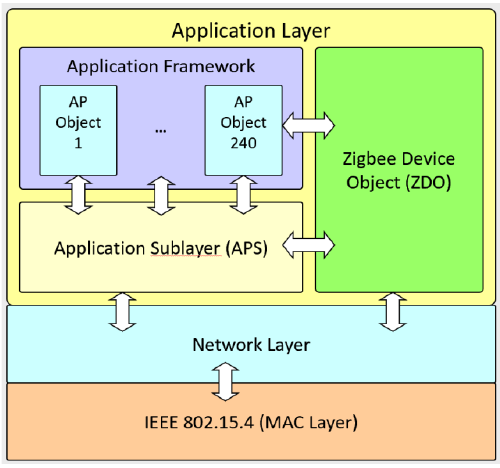
\includegraphics{images/questions/Schermata del 2023-10-19 15-32-10.png}
   % \caption{}
   \label{fig:dom7}
\end{figure}
   
Nella figura viene rappresentato il livello applicazione di ZigBee a sua volta diviso in 3 sotto-livelli:

\begin{itemize}
\item \textbf{Application Framework}: contiene fino a 240 \emph{Application Object (APO)}, ovvero applicazioni ZigBee definite e implementate dall'utente. Ogni APO è identificato in modo univoco all'interno della rete e i più semplici possono essere interrogati utilizzando il \emph{Key Value Pair (KVP) data service}.
Gli APO più complessi al contrario, possono gestire al loro interno anche uno stato più complicato; di conseguenza necessitano l'interazione con il \emph{Message data service}. Ciascun APO rappresenta un componente singolo del device (e.g., lampadina di un dispositivo o interruttore);
\item \textbf{ZigBee Device Object (ZDO)}: è un'applicazione speciale situata sull'endpoint 0 e gestisce il comportamento di un device in una rete ZigBee. 
\note{Dunque implementa le funzionalità di end-device, router o coordinator. Implementa comportamenti come rispondere a una device discovery.}
Un profilo speciale, lo \textit{ZigBee Device Profile}, descrive i cluster che devono essere supportati da ogni device ZigBee, che sono implementati dallo ZDO.
In particolare sono implementati i servizi di (device e service) discovery e binding, e come gestisce network e sicurezza. 
\begin{itemize}
   \item device e service discovery;
   
   \item binding management;
   
   \item network management;
   
   \item node management
\end{itemize}
\item \textbf{Application Support Sublayer (APS)}: è una sorta di livello di trasporto, simile a TCP, ma offre funzionalità diverse. È responsabile principalmente di fornire dati e gestire i servizi agli APO e ZDO. Inoltre, definisce:
\begin{itemize}
   \item gli endpoint: identificatori univoci degli APO che vanno da 1 a 240;
   
   \item i cluster: protocolli che definiscono un set di messaggi e comandi che i device possono usare per comunicare, ogni cluster è identificato in modo univoco tramite un cluster ID;
   
   \item profile ID e device ID.
\end{itemize}

Uno dei servizi fondamentali dell'APS è l'APS binding che permette di interconnettere l'endpoint di un nodo con uno o più endpoint di un altro nodo. Inoltre, il binding è unidirezionale e può essere gestito dallo ZDO di un coordinatore o di un router. \\
Nell'APS risiedono l'\textbf{Address Map} e la \textbf{Binding Table}.
\end{itemize}

Il \textbf{Network Layer} fornisce gestisce l'addressing, il routing e funzionalità di sicurezza (No SSL, si utilizza AES-128 o nell'APS o nel NWK); infatti gli indirizzi NWK servono per l'identificazione dei device (e APOs).
Fornisce un livello di astrazione rispetto al \textbf{MAC layer}, che opera più a basso livello astraendo dal livello fisico e occupandosi di (ri)trasmissione/ricezione dei frame, scan delle reti disponibili, unione a una rete, ecc.

\section{Topologie ZigBee}

\begin{figure}[htbp]
   \centering
   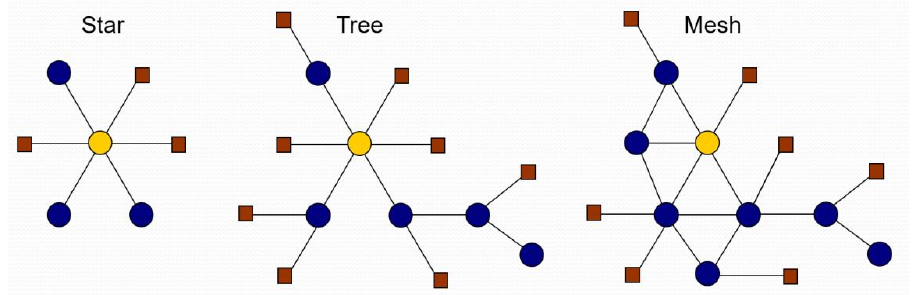
\includegraphics{images/questions/Schermata del 2023-10-19 15-34-16.png}
   % \caption{}
   \label{fig:dom8}
\end{figure}

Possiamo distinguere tre tipo di topologie di rete:

\begin{itemize}
\item \textbf{Topologia a stella}: il nodo centrale è sempre un coordinatore, mentre gli altri nodi possono essere indifferentemente router o end-device che svolgono lo stesso ruolo. Per la comunicazione utilizzano il \emph{superframe};
\item \textbf{Topologia ad albero}: sfrutta i router per ampliare la copertura della rete. Il nodo radice sarà sempre un network coordinator, i router possono assumere il ruolo di nodi intermedi attraverso i quali avvengono le comunicazioni oppure possono essere nodi foglia, mentre gli end-device possono soltanto essere nodi foglia. Inoltre, vengono supportate le funzionalità della rete multi-hop;
\note{Superframe facoltativo}
\item \textbf{Topologia mesh}: Essenzialmente è una rete p2p multi-hop, con path multipli che portano alla stessa destinazione.
Anche se possibile utilizzarlo, la comunicazione è possibile anche tra nodi anche senza affidarsi all'infrastruttura superframe, sfruttando channel sharing e meccanismi di collision avoidance.
\end{itemize}

\section{ZigBee Address Tree}

\begin{figure}[htbp]
   \centering
   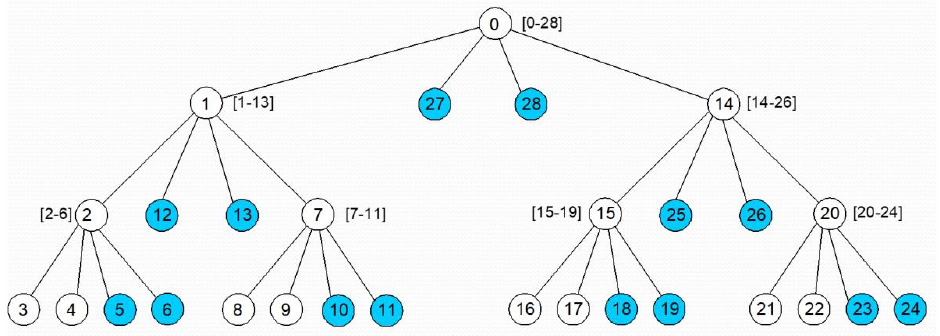
\includegraphics{images/questions/Schermata del 2023-10-19 15-35-42.png}
   % \caption{}
   \label{fig:dom9}
\end{figure}

Topologia basata su alberi viene sfruttata dal livello rete di ZigBee per assegnare l'indirizzo di rete breve basato su una politica definita dal coordinatore ZigBee. I parametri utilizzati sono:

\begin{itemize}
\item Il \textbf{massimo numero di router} che ogni router ha come figlio: \textbf{\emph{Rm}};
\item Il \textbf{massimo numero di dispositivi terminali} che ogni router ha come figlio: \textbf{\emph{Dm}};
\item La \textbf{massima lunghezza dell'albero}: \textbf{\emph{Lm}}.
\end{itemize}

Guardando l'immagine si ha una rete ad albero con \emph{Rm}=2, \emph{Dm}=2 e \emph{Lm}=3. Il coordinatore ha indice 0 e il suo figlio sinistro 1. Il numero massimo di nodi in questo esempio è 28 perché è la soglia data dai tre parametri prima descritti. Questo limita il numero di nuovi dispositivi che possono unirsi alla rete, quindi un nuovo dispositivo non può entrare nella rete se viene raggiunto il limite. L'assegnazione del range viene dato seguendo un ordine DFS.

Se il nodo 3 vuole comunicare con il nodo 25, deve inviare il pacchetto al nodo 2, ed essendo 25 fuori dal suo range esso deve mandare il pacchetto al nodo 1 (nodo padre) e per lo stesso motivo al nodo 0. Il pacchetto viene poi inviato al nodo 14 che ha nel suo range 25. Queste comunicazioni avvengono per maggioranza tra router, tranne tre, quella che porta da 14 a 25 poiché è un dispositivo terminale, ma anche quelle da 1 a 0 e da 0 a 14, visto che 0 è la root ed è un network coordinator.

\section{Tabella di binding ZigBee}

\begin{figure}[htbp]
   \centering
   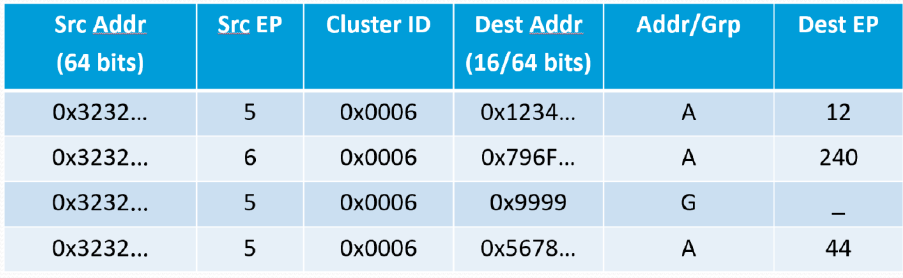
\includegraphics{images/questions/Schermata del 2023-10-19 15-37-17.png}
   % \caption{}
   \label{fig:dom10}
\end{figure}

Tabella di binding gestita dal Application Support Sublayer (APS). L'operazione di binding permette ad un end-point (APO) di un device di connettersi ad uno o più end-point su altri nodi senza conoscerne il NWK address né tantomeno l'endpoint di destinazione: il binding è unidirezionale e può essere configurato solo dal ZDO del coordinator o di un router. \\
Il binding quindi fornisce un modo di non specificare l'indirizzo di destinazione di un messaggio (\textbf{Indirect Addressing}), opposto al più canonico metodo del \textbf{direct addressing} che prevede che la sorgente indichi la tupla $\langle$\texttt{destination address}, \texttt{destination endpoint}$\rangle$ e che potrebbe essere non applicabile per dispositivi molto semplici.
In questo modo, l'invio dei messaggi presso i destinatari è totalmente delegato a router e coordinator, dove risiede la binding table, tipicamente inizializzata a tempo di configurazione della rete, e aggiornata solo su esplicita richiesta dello ZDO di coordinator e router.



Le due primitive principali utilizzate per il binding sono BIND e UNBIND che servono rispettivamente per creare una nuova entry nella tabella di binding locale e per eliminarla. \\
La entry mantiene l'indirizzo sorgente (MAC a 64 bit), l'endpoint sorgente, l'identificatore del cluster, l'indirizzo a 64 bit di destinazione (o indirizzo 16 bit multicast\footnote{NON il NWK address a 16bit!!!}) e l'endpoint di destinazione. Questa tabella viene salvata in modo persistente nell'APS del coordinatore di ZigBee e/o di un altro router: viene caricata su esplicita richiesta del ZDO.

Un messaggio viene inoltrato alla/e destinazione/i trovando le entry che nella binding table matchano la tupla $\langle$\texttt{source address}, \texttt{source endpoint}, \texttt{clusterID}$\rangle$ del messaggio in arrivo. 
In caso di multipli match, avverrà una comunicazione multicast e il messaggio sarà inoltrato alle multiple destinazioni.
\note{In figura per la tupla $\langle 0x3232...,5,0x0006 \rangle$ abbiamo più entry corrispondenti a più destinazioni.}
\note{Se non ci sono match, il messaggio viene scartato.}

\section{Diagramma di configurazione e interconnessione delle luci}

\begin{figure}[htbp]
   \centering
   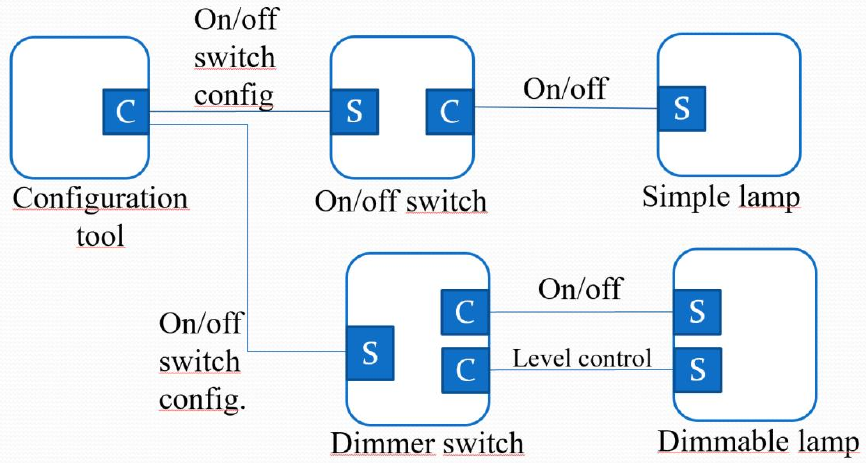
\includegraphics{images/questions/Schermata del 2023-10-19 15-41-05.png}
   % \caption{}
   \label{fig:dom11}
\end{figure}

Esempio di utilizzo della ZigBee Cluster Library (ZCL) che contiene le specifiche e i framework per i cluster implementati dalle applicazioni degli utenti. \ul{Per cluster si intende collezione di comandi e attributi relativi a un \textit{dominio funzionale}} (che definiscono un'interfaccia di una specifica funzionalità).
Tali comandi sono definiti seguendo un modello client-server, dove il dispositivo che salva gli attributi mantenendo uno stato interno è un server mentre i dispositivi che manipolano gli attributi sono client.\\
{\ns La ZCL definisce anche dei messaggi per:
\begin{itemize}
   \item Leggere/scrivere attributi
   \item Configurare un report e leggere una risposta in formato report
   \item Scoprire ID e tipi degli attributi supportati da un server 
\end{itemize}}

Nella figura si parla di cluster nel dominio funzionale \emph{Lighting} in cui si vuole configurare un insieme di APO con uno switch ON/OFF connesso con una ``simple lamp" e un ``dimmer switch" connesso ad una ``dimmable lamp", che sono i cluster. Il configuration tool crea l'associazione tra i due APO funzionando come un client che imposta la configurazione del dispositivo di switch in modo che quando la lampada sia accesa o spenta questo possa essere visto nel dispositivo corrispondente. Il configuration tool imposta una tabella di routing nel coordinator conoscendo l'indirizzo dei dispositivi e dei relativi APO.

\section{Duty Cycle I}

\begin{figure}[htbp]
   \centering
   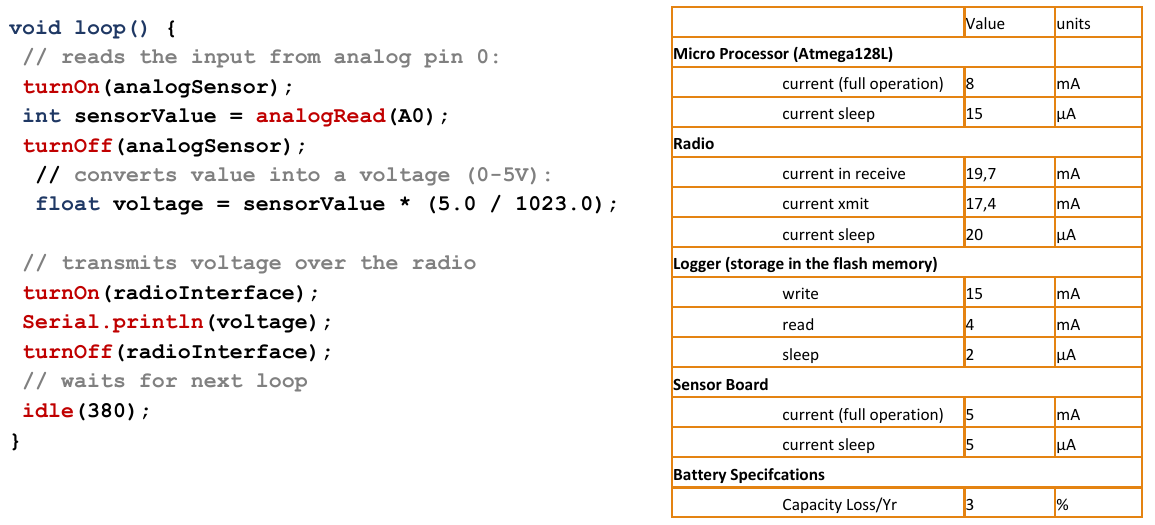
\includegraphics{images/questions/Schermata del 2023-10-19 15-42-33.png}
   % \caption{}
   \label{fig:dom12}
\end{figure}

Il codice in figura mostra un esempio di un programma Arduino, in cui ogni componente viene accesso, utilizzato e poi successivamente subito spento per cercare di ottimizzare il consumo energetico del device su cui questo codice è installato. 
% Infatti il problema del consumo energetico è un problema centrale in ambito IoT, in quanto tali dispositivi hanno un ciclo di vita finito, dopo il quale devono essere sostituiti.
Per aumentare il lifetime è necessario ottimizzare il duty cycle di ogni componente, ovvero il rapporto tra il \ul{tempo di attività e e il periodo}\footnote{valore arbitrario maggiore o uguale del tempo di attività, onde evitare complicazioni nei calcoli}.
Il duty cycle complessivo di un dispositivo è pari alla somma dei duty cycle di ogni singolo componente, assumendo che i cicli di operatività siano ``disgiunti'' e alcune semplificazioni sull'effettivo istante di ON/OFF.
Ad esempio, \textit{Duty cycle = 1\%} implica che il device sia accesso solo per il 1\% del tempo totale, e spento per il restante 99\%.

Negli esercizi si considera il tempo richiesto per ciascuna operazione di CPU/Radio/Sensore/ecc. (in figura non riportato), e si rapporta al periodo complessivo (in figura il periodo \textbf{non} è 380!).

Per calcolare i consumi energetici, si fa riferimento alla tabella dei consumi tipicamente fornita per ogni dispositivo IoT. Data la capacità della batteria equipaggiata, è possibile calcolare l'expected lifetime, moltiplicando il duty cycle per il la corrente consumata di ciascun componente, sommando i risultati, e dividendo la capacità della batteria per tale numero.

\note{
   Duty cycle CPU = $1\% = 0.01$\\
   $0.01\cdot 8mA + 0.99\cdot 0.015mA = 0.095mA$\\
   $2000mAh / 0.095mA = 21052 ore = 2.4 anni$}


\section{Duty Cycle II}

\begin{figure}[htbp]
   \centering
   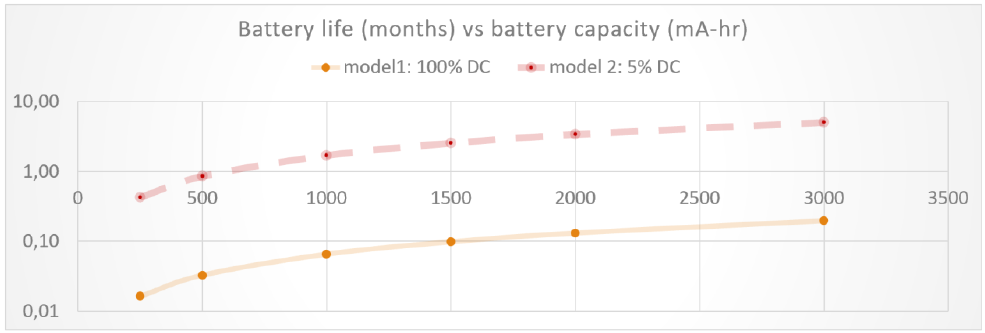
\includegraphics{images/questions/Schermata del 2023-10-19 15-44-53.png}
   % \caption{}
   \label{fig:dom13}
\end{figure}

{\ns In questo diagramma si ha il confronto tra due modelli con duty cycle differenti:
\begin{itemize}
\item Il primo modello ha un DC pari al 100\%, ovvero con ogni componente del device sempre in funzione;
\item Il secondo modello ha un DC pari al 5\%, ovvero con un tempo di inattività delle sue componenti pari al 95\%.
\end{itemize}}

Come è possibile osservare dal grafico, il secondo modello ha un tempo di vita della batteria maggiore rispetto al primo a parità di capacità della batteria, questo perché il tempo di utilizzo limitato incrementa sicuramente il tempo di vita di un sensore, ma d'altro canto richiede che le attività delle varie componenti del device siano schedulate in modo efficiente, per rispettare le performance attese.

È necessario fare il tuning dei parametri del duty cycle affinché non solo il dispositivo funzioni efficientemente, ma che tale duty cycle gli permetta di fare sampling in modo produttivo e di funzionare correttamente. (e.g. Un sensore della temperatura per una stanza in una casa, non può fare sampling ogni due giorni)
 
\section{Embedded programming I}

\begin{figure}[htbp]
   \centering
   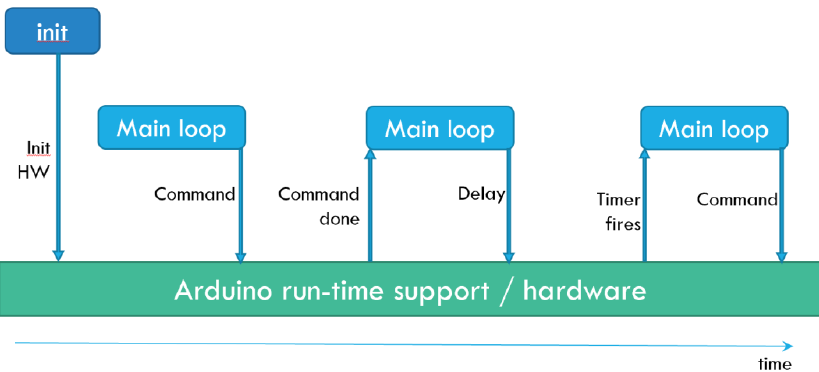
\includegraphics{images/questions/Schermata del 2023-10-19 15-45-55.png}
   % \caption{}
   \label{fig:dom14}
\end{figure}

Arduino è single threaded e il suo flow di esecuzione è una singola loop function che può invocare altre funzioni.
Non c'è la sospensione del thread, dunque operazioni di I/O fanno attendere il main thread finché non sono completate.
Gli step dell'esecuzione sono i seguenti:

\begin{enumerate}
\item Il device invoca la funzione \texttt{init} che permette l'inizializzazione del dispositivo stesso e abilita la comunicazione con i componenti hardware;
\item Viene invocato il main \texttt{loop()} rappresentante il ciclo delle operazioni da svolgere periodicamente.
\item Nell'esempio viene inviato un comando a una componente hardware; quando è stato eseguito l'Arduino RTS invia un segnale di terminazione del comando e restituisce il controllo al main loop;
\item Se il carico di lavoro attivo è stato compiuto si può invocare in modo esplicito la funzione \texttt{delay} che invia un comando ad un timer sospendendo la CPU finché il timer riattiva il \texttt{main loop} con un segnale (\texttt{timer fires}).
\end{enumerate}

\section{Embedded programming II}

\begin{figure}[htbp]
   \centering
   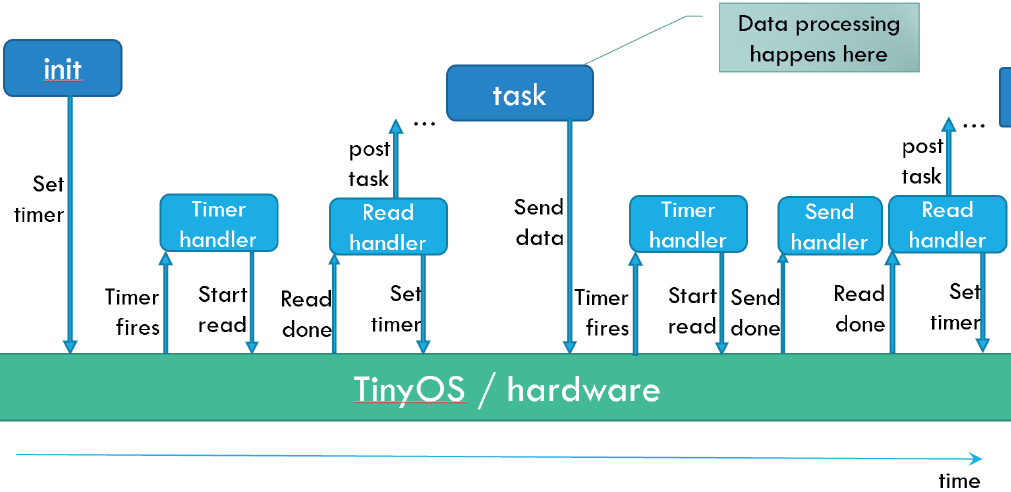
\includegraphics{images/questions/Schermata del 2023-10-19 15-47-07.png}
   % \caption{}
   \label{fig:dom15}
\end{figure}

In figura viene mostrato come TinyOS gestisce il software di un device, progettato per gestire principalmente eventi asincroni attraverso 3 concetti fondamentali:

\begin{itemize}
\item \textit{Comandi}: utilizzati per programmare e comunicare con l'hardware.
\item \textit{Eventi}: astraggono interruzioni hardware come una sorta di upcall.
\item \textit{Task}: definiti per gestire attività differenti e indipendenti. Quando un task è terminato e non ce ne sono altri da eseguire allora la CPU passa in \texttt{idle mode};
\end{itemize}

\begin{enumerate}
   \item La funzione \texttt{init} dopo aver inizializzato il device setta un timer e un handler da eseguire allo scadere.
   \item \texttt{timer handler} ---definita dall'utente oppure fornita dal RTS--- può, ad esempio, richiedere una lettura da un sensore; 
   \item Terminata la lettura, un \texttt{read handler} gestirà questo evento schedulando un nuovo task (ad alto livello) che potrà eseguire operazioni più complesse sui dati.
   \item Terminate le operazioni sui dati, questi saranno inviati all'hardware e verrà settato nuovamente un timer, che farà ripartire il ciclo degli eventi come successivamente alla funzione di init.
   \item TinyOS gestisce l'esecuzione di un singolo handler alla volta alla volta e infatti dovrebbero essere brevi: più interruzioni simultanee potrebbero causare seri problemi di concorrenza.Tuttavia è possibile che un'operazione hardware in corso (come l'ultima lettura in figura) possa essere interrotta da un'altra ``upcall''.
\end{enumerate}
I comandi invocati dagli handler non devono riguardare il componente HW che ha triggerato l'handler, onde evitare stati inconsistenti.

Con questo modello una task ``non aspetta mai'' che venga eseguita lettura o scrittura hardware, e può essere pre-empted solo da degli eventi; non sarà lei a richiedere esplicitamente di andare in idle, come nel caso di Arduino con il comando \texttt{delay}.

\section{Interruzioni Arduino}

\begin{figure}[htbp]
   \centering
   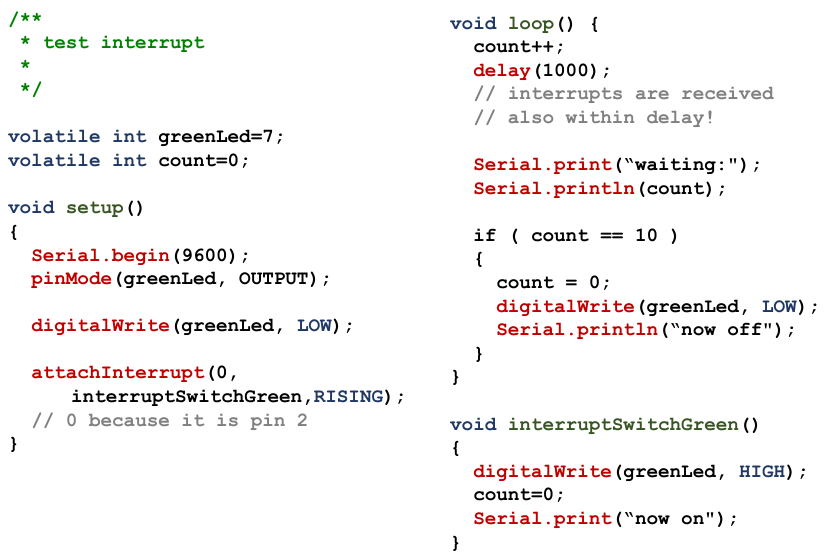
\includegraphics{images/questions/Schermata del 2023-10-20 11-32-10.png}
   % \caption{}
   \label{fig:dom16}
\end{figure}

Nel codice si può osservare il meccanismo delle interruzioni di Arduino che, come in TinyOS, permette di gestire eventi asincroni. Le interruzioni possono essere di tre tipi: \textit{esterne}, \textit{timer} o di \textit{dispositivo}. 
Esse vengono gestite dal RTS. In questo caso osserviamo come si ha una funzione di \lstinline{loop} principale in cui c'è un'attesa fissa che viene seguita da una scrittura digitale. All'occorrenza di un'interruzione \textit{esterna} è possibile come in questo caso definire un comportamento predefinito attraverso la funzione \lstinline{attachInterrupt(interrupt\#, funct-name, mode)} nella funzione di \lstinline{setup()}. Le modalità sono le seguenti:

\begin{itemize}
\item \textbf{RISING}: l'interruzione avviene quando il pin passa da un valore LOW ad un valore HIGH;
\item \textbf{FALLING}: l'interruzione avviene quando il pin passa da un valore HIGH ad un valore LOW;
\item \textbf{CHANGE}: l'interruzione avviene quando il pin cambia stato;
\item \textbf{LOW}: l'interruzione avviene quando il pin ha uno stato basso. Non necessariamente un cambio di stato, se rimane LOW l'interruzione avviene di nuovo;
\item \textbf{HIGH}: l'interruzione avviene quando il pin ha uno stato alto. Non necessariamente un cambio di stato, se rimane HIGH l'interruzione avviene di nuovo.
\end{itemize}

Nella figura, \lstinline{greenlLed = 7} definisce il pin 7 come il pin di output per il led verde, mentre \lstinline{attachInterrupt(0, interruptSwitchGreen, CHANGE)} definisce che l'interruzione avverrà sul pin 2 (corrispondente all'interruzione 0) e che la funzione \lstinline{interruptSwitchGreen} verrà eseguita quando il pin passerà da \lstinline{LOW} ad \lstinline{HIGH} (il cambio di stato è \lstinline{RISING}). \lstinline{interruptSwitchGreen} è una funzione che cambia lo stato del led verde.
\lstinline{Serial.begin(9600)} setta il data rate di trasmissione a 9600bit/s

\note{Saper spiegare il resto del codice a voce}

\section{SMAC}

\begin{figure}[htbp]
   \centering
   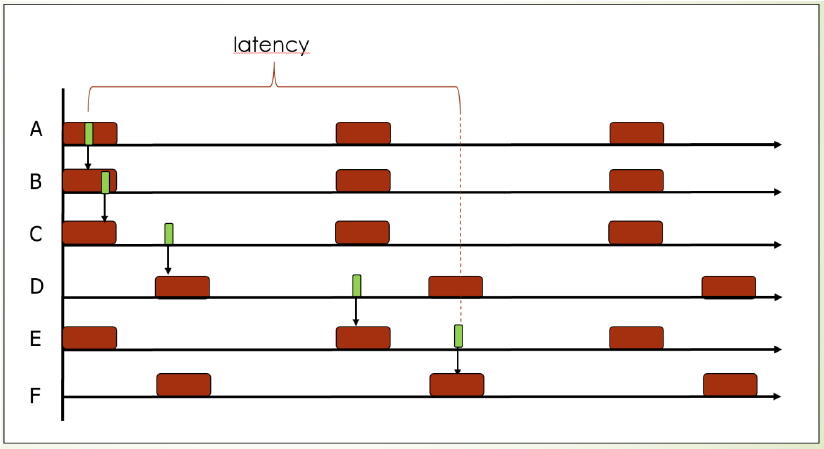
\includegraphics{images/questions/Schermata del 2023-10-20 11-35-40.png}
   % \caption{}
   \label{fig:dom17}
\end{figure}

Lo schema in figura rappresenta lo scambio di messaggi tramite l'utilizzo del protocollo SMAC, un protocollo MAC (\textit{Medium Access Control}) per le reti wireless multihop.
SMAC è utilizzato in 802.11, mentre in 802.15.4 si utilizza il \textbf{polling} (beacon).
In questo protocollo i nodi utilizzano una sincronizzazione locale per poter comunicare con i propri vicini, ottenuta tramite lo \ul{scambio di messaggi \texttt{SYNC} che permettono di sincronizzare i duty cycle} ---della radio--- dei dispositivi in modo che si accendano nello stesso momento.

Qualora un nodo voglia inviare a un ricevente che non è sincronizzato con il suo stesso ciclo, dovrà comunicare nel time slot del nodo ricevente, eventualmente svegliandosi fuori dal suo slot predefinito.

Visto che le comunicazioni avvengono nel timeframe del ricevente è possibile che si vengano a creare delle collisioni, per questo motivo prima di inviare un messaggio viene effettuato un controllo \textit{Carrier Sense} per comprendere se il canale sia occupato o meno, causando ritardi nella trasmissione. Se vengono ricevuti o un \texttt{RTS} (Request To Send) o un \texttt{CTS} (Clear To Send) la trasmissione viene lasciata attiva perché questa sia terminata.

Questo protocollo ha due problemi principali, il primo, la \textbf{latenza}, dovuta alla difficoltà nel sincronizzare molteplici nodi distanti (resa accettabile da cluster di nodi vicini che invece riescono a sincronizzarsi), mentre il secondo è la qualità degli \textbf{orologi interni} dei device (spesso cheap), che possono portare a oscillazioni nella misurazione del tempo e dunque a desincronizzazioni.

\note{Inoltre il CSMA/CA usato ha i problemi di \textit{hidden/exposed terminal}.}

\section{BMAC}

\begin{figure}[htbp]
   \centering
   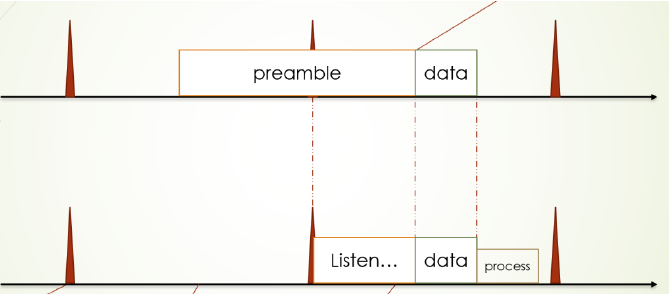
\includegraphics{images/questions/Schermata del 2023-10-20 11-36-52.png}
   % \caption{}
   \label{fig:dom18}
\end{figure}

Lo schema in figura rappresenta lo scambio di dati attraverso il protocollo BMAC. Il protocollo BMAC è un protocollo \emph{medium access control} che riduce la complessità del protocollo SMAC, in quanto richiede la configurazione di un unico parametro, stabilito out-of-band.

In questo protocollo il mittente può inviare un messaggio che contiene un lungo preambolo (preamble), in qualsiasi momento. Al contrario il ricevente attiva la radio periodicamente controllando se c'è un preamble che deve essere catturato (preamble sampling) basandosi sulla modalità \emph{Low-Power Listening (LPL)}.\\
Questi preamble dovranno avere una lunghezza maggiore rispetto all'intervallo che avviene tra un campionamento ed un altro e un punto a sfavore risiede nel fatto che il ricevente deve attendere la fine del preamble prima di ricevere i dati.
\note{Viene da chiedersi se un nodo prima di inviare un preambolo debba provare ad ascoltare per  capire se il canale non sia già occupato, o se invece sia legato al spike rosso indicante il wake-up}

Il protocollo permette ai receiver di utilizzare meno energia, a scapito dei consumi maggiori del sender; dunque BMAC trova un'utile applicazione in scenari dove ci sono più receiver e pochi sender.

\section{Device Lifetime e BMAC}

\begin{figure}[htbp]
   \centering
   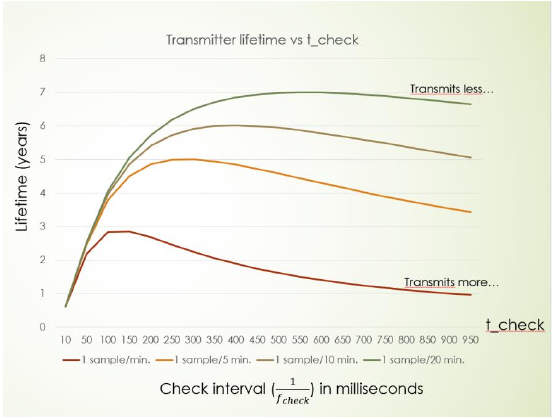
\includegraphics{images/questions/Schermata del 2023-10-20 11-37-09.png}
   % \caption{}
   \label{fig:dom19}
\end{figure}

Il diagramma in figura mostra l'andamento del tempo di vita di un \textbf{trasmettitore} mettendo in rapporto la frequenza di invio dei sample, il tempo fra i wake-up ($t_check$), e gli anni di vita di un dispositivo. Si può osservare come ad una frequenza di campionamento maggiore (per esempio 1 sample al minuto - linea rossa) il tempo di vita sia molto breve, addirittura inferiore ai 3 anni, mentre con un campionamento meno frequente (per esempio 1 sample ogni 20 minuti - linea verde), il tempo di vita aumenta sensibilmente raggiungendo un massimo che supera sfiora 3 volte il tempo di vita usando il campionamento con la linea rossa.

%The node lifetime depends on the check interval (of preamble sampling) and the total amount of traffic in the network cell.
Ciò che è interessante è vedere come indipendentemente dalla frequenza dei sample, il trend sia comunque decrescente oltre un certo $t_{check}$, il tempo fra un risveglio e l'altro, indicante anche la lunghezza del preambolo da mandare.


\note{
Tali valori sono ottenuti attraverso le seguenti formule che formalizzano il tempo di vita di un trasmettitore:

\begin{itemize}
\item $DC_{tx}=f_{data}\cdot(t_{preamble}+t_{data})$

\item dove abbiamo $f_{data}$ frequenza di invio dei dati, $t_{preamble}$ l'intervallo di invio del preamble, $t_{data}$ l'intervallo di invio dei dati.
\item $DC_{check}=f_{check}\cdot t_{check}$

\item dove abbiamo $f_{check}$ la frequenza di sampling, $t_{check}$ l'intervallo di sample frequency
\item $ET(t)=t\cdot(p_{tx}DC_{tx}+p_{tx}DC_{check}+p_{sleep}*(1-DC_{tx}-DC_{check}))$


\item dove $p_{tx}, p_{sleep}$ rappresentano rispettivamente il consumo energetico durante la fase di trasmissione e il consumo energetico durante la fase di riposo
\end{itemize}
\textred{TODO verifica formule se sono scritte bene}
}


\section{XMAC/BMAC}

\begin{figure}[htbp]
   \centering
   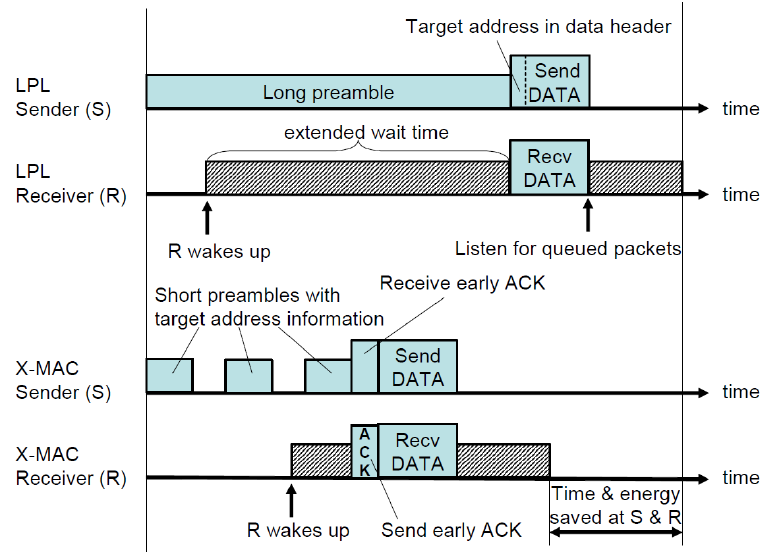
\includegraphics{images/questions/Schermata del 2023-10-20 11-48-12.png}
   % \caption{}
   \label{fig:dom20}
\end{figure}

Il protocollo X-MAC è un'evoluzione del protocollo B-MAC che mira a ridurre l'impiego di lunghi preamble vuoti. 

Per fare ciò il protocollo permette al ricevente di fermare l'invio del preamble inviando un ACK:\\
quando un receiver trova il suo ID all'interno di uno dei preamble brevi inviati da un sender allora questo invierà un early ACK al sender che sospenderà l'invio dei preamble e invierà i dati al ricevente che è pronto a riceverli. 
\note{Il ricevente dopo la ricezione dei dati non spegnerà immediatamente la componente radio per permettere ad altri eventuali nodi di inviargli dati nel caso in cui abbiano trovato il canale precedentemente occupato.}

Nell'immagine si può vedere come in XMAC nella fase di trasmissione invia un preambolo breve contenente informazioni sull'indirizzo dei target, quando il ricevente si sveglia e cattura il preambolo breve replica con un ACK che permette al mittente di iniziare l'invio dei preamboli brevi e di iniziare ad inviare i frame con i dati.

BoX-MAC è un'ulteriore sviluppo di XMAC, in cui si sostituisce il preambolo con l'invio ripetuto dei dati (insieme alle informazioni sui destinatari).
\note{È adatto per applicazioni in cui i dati sono piccoli e la latenza è critica.}

\section{IEEE 802.15.4 superframe}

\begin{figure}[htbp]
   \centering
   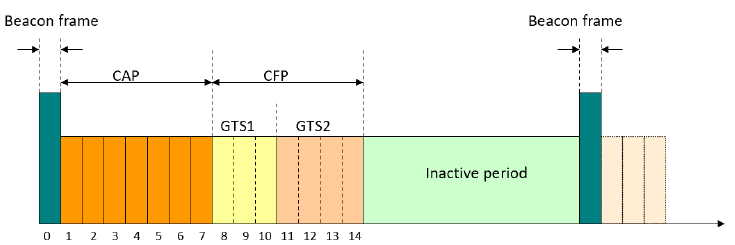
\includegraphics{images/questions/Schermata del 2023-10-20 11-49-03.png}
   % \caption{}
   \label{fig:dom21}
\end{figure}

L'immagine mostra il servizio di channel access per il livello MAC del protocollo IEEE 802.04.15. Abbiamo due tipi di accesso a livello MAC:
{
   \ns
   \begin{enumerate}
      \item con superframe structure;
      \item senza superframe structure;
      \end{enumerate}
      
      }

Nello specifico l'immagine mostra un channel access con superframe structure, utilizzato solitamente nelle topologia a stella o nelle topologie peer-to-peer, ma con struttura ad albero.
In caso di reti \textit{non-beacon enable}, la comunicazione avviene senza superframe structure, con un protocollo unslotted \texttt{CSMA-CA};
il coordinator è sempre pronto a ricevere dati da un end-device mentre la trasmissione da end-device a coordinator è poll-based: l'end-device si sveglia periodicamente e interroga il coordinator per i messaggi in attesa.

Un superframe è composto da due parti, una attiva e l'altra inattiva. 
Tutte le comunicazioni avvengono durante il periodo attivo, mentre in quello inattivo i nodi possono andare in idle.  

La parte attiva, in cui è possibile comunicare è composta a sua volta da 15 time frame della stessa dimensione, di cui il primo di questi è detto beacon frame ed è inviato dal PAN coordinator. 
Il beacon frame serve per sincronizzare i dispositivi collegati, per identificare il PAN e descrivere la struttura del superframe. 

La comunicazione vera e propria tra l'end device e il coordinatore (\ul{non con i router}) avviene nella restante parte del periodi di attività, che è divisa in due parti:

\begin{itemize}
\item \textbf{Contention Access Period (CAP)}: il dispositivo compete per accedere al canale utilizzando il protocollo standard slotted CSMA/CA. 
Un dispositivo che vuole trasmettere i frame dati prima deve aspettare il beacon frame e dopo randomicamente seleziona uno slot temporale per la sua trasmissione: se seleziona uno slot occupato da un'altra comunicazione allora proverà a selezionarne un altro, altrimenti attenderà il successivo superframe.\\
Una volta iniziata la trasmissione, il sender tiene il canale occupato fino alla fine del frame.
\note{\ul{Il CAP period deve essere composto da almeno uno slot}, per permettere a nuovi device di unirsi alla rete}

\item \textbf{Contention Free Period (CFP)}: opzionale e utilizzato per applicazioni a bassa latenza o che richiedono uno specifico bandwidth. Il coordinatore PAN può assegnare porzioni di questa parte chiamati \textbf{GTS (Guaranteed Time Slot)} a specifiche applicazioni.
\note{In caso ci siano più richieste di GTS di quante ne siano disponibili, il coordinatore PAN può assegnare i GTS in base a priorità o in base a un algoritmo di scheduling, altrimenti risponde ai richiedenti ``picche'' \smiley.}
\end{itemize}

\section{Trasferimento dei dati IEEE 802.15.4}

\begin{figure}[htbp]
   \centering
   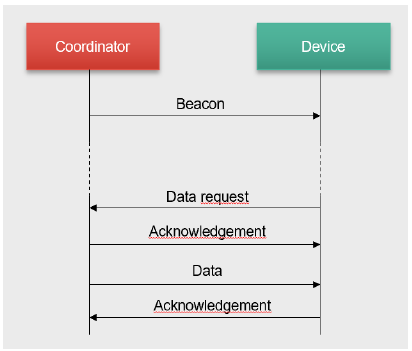
\includegraphics{images/questions/Schermata del 2023-10-20 11-49-16.png}
   % \caption{}
   \label{fig:dom22}
\end{figure}

Il sequence diagram nell'immagine mostra il trasferimento di dati da un \textit{coordinator} $\longrightarrow$ \textit{device} in una rete \textbf{beacon enabled}.
\\Esistono 3 diversi modelli di trasferimento dati: end-device al coordinatore, coordinatore all'end-device, peer-to-peer. 

\begin{itemize}
   \item coordinator a end device:\\
   il coordinator indica nel network beacon che esiste un messaggio per l'end device.\\
   Gli end device restano per la maggior parte del tempo in sleep mode, ma periodicamente si svegliano per controllare messaggi pending, e se ce ne sono li richiedono usando uno slot nel CAP.\\
   Il coordinator invia il pending message utilizzando anch'esso un protocollo CSMA-CA con slot all'interno del CAP. Una volta ricevuto il frame, il dispositivo può riconoscere la ricezione trasmettendo un ACK in uno slot temporale successivo;
   \item \note{end device a coordinator: il dispositivo attende il beacon di rete per sincronizzarsi con il superframe. Dopodiché, se possiede un GTS lo usa direttamente, altrimenti trasmette il data frame al coordinator utilizzando protocollo standard CSMA-CA in uno dei frame del CAP (Contention Access Period). Il coordinator riconosce la ricezione con successo trasmettendo un ACK in uno slot temporale successivo;}
\item \note{peer-to-peer: nel caso uno dei due dispositivi coinvolti nella comunicazione sia un end device allora si utilizza uno dei due protocolli sopra. Al contrario se entrambi i device sono coordinator e ognuno possiede il proprio network beacon, allora il mittente del messaggio deve sincronizzarsi prima con il network beacon del ricevente e comportarsi poi come un end device. }
\end{itemize}

\section{IEEE 802.15.4}

\begin{figure}[htbp]
   \centering
   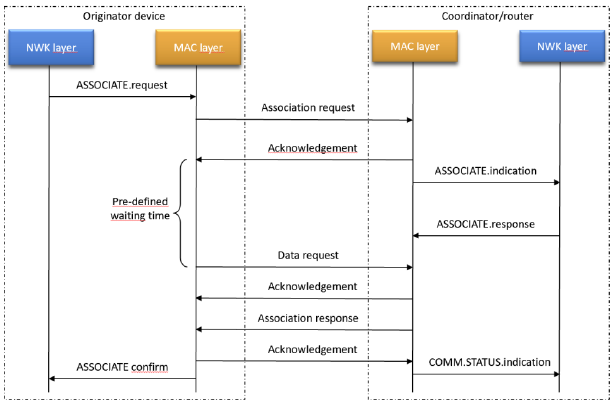
\includegraphics{images/questions/Schermata del 2023-10-20 11-49-37.png}
   % \caption{}
   \label{fig:dom23}
\end{figure}

Il sequence diagram in figura rappresenta una richiesta di servizio ASSOCIATE, che viene invocato da un dispositivo che desidera associarsi con un PAN di cui ha l'identificativo da una invocazione preliminare del servizio SCAN. 

\begin{enumerate}
   \item La primitiva \texttt{ASSOCIATE.request} prende come parametro l'identificatore di una PAN, l'indirizzo del coordinatore e l'indirizzo IEEE esteso a 64 bit del dispositivo stesso.
   \note{La primitiva invia un messaggio di richiesta di associazione al coordinatore e, poiché la procedura di associazione è pensata per le reti abilitate al beacon, il messaggio di richiesta di associazione viene inviato durante il periodo CAP utilizzando il protocollo CSMA-CA.}
   \item 
   Il coordinatore invia un messaggio di ACK in cui riconosce la ricezione del messaggio ma non per questo l'associazione alla PAN è avvenuta con successo.
   \item Il coordinatore, attraverso la primitiva \texttt{ASSOCIATE.indication}, passa la richiesta al livello di rete dove viene effettuata la decisione sull'associazione:
   in caso questa sia accettata viene selezionato un indirizzo a 16 bit che il dispositivo utilizzerà in seguito al posto di quello IEEE da 64 bit.
   \item Il livello rete ritorna con la primitiva \texttt{ASSOCIATE.response} al livello MAC che prende come parametro l'indirizzo a 64 bit del dispositivo, il nuovo indirizzo a 16 bit e lo stato della richiesta.\\
   Il coordinatore genera così un pending message con la risposta dell'associazione.
   \item \ul{Dopo un periodo definito di attesa} il dispositivo fa una \textit{Data request} a cui corrisponde un ACK del coordinatore e a seguire il messaggio contenente la risposta dell'associazione, corrisposto da un ACK inviato dal device al coordinator
   \note{Deve essere il device a contattare il coordinator perché non conosce ancora il suo NWK address e il coordinator dovrebbe inserire tale address per inviargli un messaggio tramite il beacon.}
   \item Lato dispositivo quindi viene invocata la primitiva \texttt{ASSOCIATE.confirm} verso il livello rete mentre lato coordinatore viene emesso \texttt{COMM-STATUS.indication} per informare il livello superiore che il protocollo di associazione si è concluso (con successo o con un codice di errore).
\end{enumerate}

\section{Energy harvesting}

\subsection{Explain the difference between an harvest-use and an harvest-store-use architecture}

Nell'architettura \textbf{Harvest-Use} si ha un modello di harvesting diretto in cui non viene fornito nessun buffer energetico per questo l'energia accumulata viene immediatamente consumata. Questo comporta due principali svantaggi:
{\ns\begin{itemize}
   \item Spreco di energia quando quella prodotta è minore di quella consumata;   
   \item Spegnimento del dispositivo quando viene prodotta meno energia di quella consumata.
\end{itemize}}
Tale modello può funzionare in caso solo di fonti di energia ---molto--- prevedibili, o di carico di lavoro statico o facilmente adattabile.
   
      
Nel caso dell'architettura \textbf{Harvest-Store-Use} viene introdotto un buffer che permette la raccolta dell'energia in eccesso per usi futuri. 
Semplificazioni del modello potrebbero non tenere conto dell'efficienza di carica e degli energy leaks.
In base al materiale della batteria (\texttt{SLA}, \texttt{NiCD}, \texttt{NiMH}, \texttt{Li-on}, o supercapacitors) è possibile stimare alcuni dei comportamenti della batteria nel tempo.



\subsection{Explain the classification of sources in terms of controllability and predictability}
\begin{enumerate}
   \item \textbf{Controllabile} fornisce una raccolta di energia quando è richiesta
   \note{Self-powered flashlight, girando una manovella la luce si accende.}
   \item \textbf{Parzialmente controllabile} produce energia in modo limitato dall'ambiente %mentre le sorgenti di energia 
   \note{Sorgente di energa RF (energia a radiofrequenza) può fornire energia a RFID, ma non si possono controllare l'intensità di propagazione nella stanza (non possiamo garantire con precisione come questa si distribuirà nello spazio)}
   \item \textbf{Non controllabili} non possono essere attivate su richiesta
   \begin{enumerate}
      \item \textbf{prevedibili}: hanno dei modelli di utilizzo che ne descrivono la disponibilità
      \note{Sole}
      \item \textbf{imprevedibili}: indovina.
      \note{Terremoti}
   \end{enumerate}
\end{enumerate}
Le sorgenti più interessanti e maggiormente oggetto di studio sono quelle \textit{non} controllabili e prevedibili, in quanto permettono di avere un modello di harvesting più preciso e di conseguenza un modello di consumo più efficiente.

Il modello di Kansal tuttavia non richiede conoscenza sulla futura produzione di energia: le sorgenti devono essere ---anche solo in parte--- prevedibili, ma la stima di produzione energetica futura si basa esclusivamente sulle precedenti osservazioni;
Nonostante ciò il modello benificia da una maggior accuratezza in caso esistano dei modelli più avanzati di previsione.


\subsection{Explain the concept of energy neutrality}
Mentre il goal principale anni fa era di massimizzare la durata della batteria, oggi si cerca di ottenere la \textbf{neutralità energetica}: una produzione di energia che permette di ottenere lo stesso livello di performance per tutta la durata di un intervallo di tempo, i.e. la produzione e il consumo sono bilanciati e sostenibili nel tempo.

Kansal la formalizza stabilendo che $B(K+1) \geq B(1)$, ovvero la batteria al termine del periodo $K+1$ deve avere almeno la stessa carica di quella iniziale.


{Ci sono due aspetti chiave
\begin{itemize}
   \item \textbf{Energy-Neutral Operation}:\\
   Scegliere le operazioni da eseguire in modo che, in qualunque time frame, l'energia usata sia sempre inferiore di quella prodotta.
   \item \textbf{Maximum Performance}:\\
   Assicurando l'operatività energy-neutral (scritta sopra), determinare qual è il massimo livello di performance che si può ottenere in un dato ambiente di harvesting.
\end{itemize}
}

\section{Consumo di energia con buffer}

\begin{figure}[htbp]
   \centering
   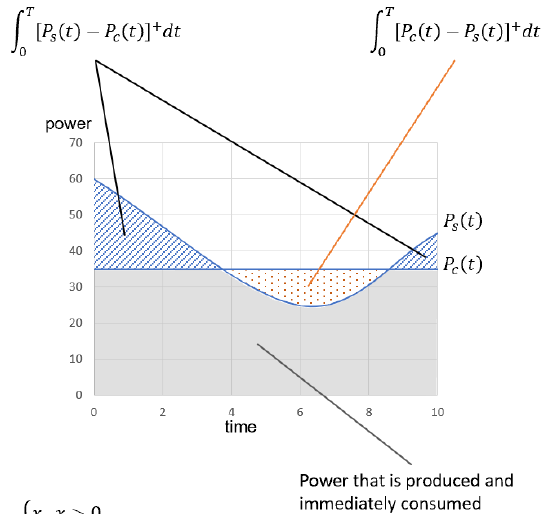
\includegraphics{images/questions/Schermata del 2023-10-20 11-54-15.png}
   % \caption{}
   \label{fig:dom25}
\end{figure}

Rappresentazione grafica del modello \textbf{Harvest-Store-Use} in cui si hanno le due funzioni che rappresentano l'energia prodotta e quella consumata, e gli integrali rappresentano l'energia che viene immediatamente consumata appena prodotta (caso in cui $consumo > produzione$) oppure l'energia che viene immagazzinata (caso in cui $produzione > consumo$). In questo modello si considera un buffer ideale senza perdite e con capacità infinita.

Per ottenere l'energy neutrality dobbiamo garantire che l'area azzurra sia maggiore dell'area arancione, in modo da consentire di mantenere il dispositivo attivo anche quando l'energia prodotta è inferiore rispetto al consumo.\\
Inoltre dobbiamo anche massimizzare l'energia disponibile, per garantire le migliori performance possibili.

Per far ciò, Kansal formalizza il problema come un problema di ottimizzazione risolubile tramite la programmazione lineare, in cui si cerca di massimizzare l'utility del dispositivo, ovvero la somma delle utilità di tutte le operazioni eseguite\footnote{duty cycle per Kansal, task nel task-based model}, avendo come vincolo che il consumo di tali operazioni non ecceda l'energia disponibile.

\section{Esercizio harvesting}

\begin{figure}[htbp]
   \centering
   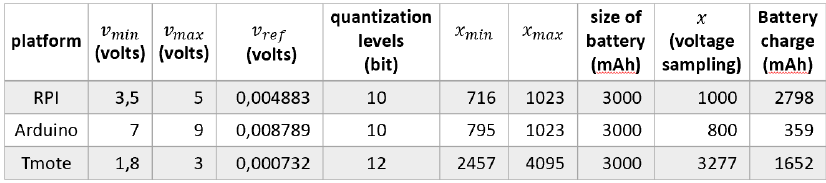
\includegraphics{images/questions/Schermata del 2023-10-20 11-56-49.png}
   % \caption{}
   \label{fig:dom26}
\end{figure}

$v_{max}$ indica la tensione fornita dalla batteria a piena carica ($B_{max}$), mentre $v_{min}$ corrisponde alla tensione fornita con la carica minima ($B_{min}$) che consente al dispositivo di funzionare.
Notare che tale carica minima, \textit{non} è una proprietà della batteria, bensì del sistema.

I dati rappresentati su $d$ bit $x_{min}$ e $x_{max}$ (e $x$ per un generico voltaggio $v$) che vengono letti dal ADC che ha in input il voltaggio, possono essere stimati matematicamente:
\begin{align}
    x_{max} &= 2^d -1\\
    x_{min} &= \left\lfloor\frac{v_{min}}{v_{max}}(2^d - 1)\right\rfloor\\
    x &= \left\lfloor\frac{v}{v_{max}}(2^d - 1)\right\rfloor
\end{align}

Il reference voltage $v_{ref}$ si calcola dividendo $v_{max}$ per il massimo intero rappresentabile con i bit dell'ADC ($2^d -1 = x_{max}$), e indica quanto ``pesa" un singolo bit.

Le ultime due colonne propongono un esempio di lettura di $x$ dall'ADC e calcolo del corrispondente livello di batteria, assumendo ---per comodità di calcolo--- che $B_{min} = 300mAh$, con la seguente formula:
\begin{align}
    B&= B_{min} + \frac{B_{max}-B_{min}}{x_{max} - x_{min}}(x-x_{min})
\end{align}
Tale formula assume una relazione lineare fra il voltaggio e la capacità della batteria, che è una approssimazione accettabile anche se in realtà dipende dalla batteria.
\begin{paracol}{2}
    \colfill
    Inoltre è opportuno osservare che il voltaggio della batteria decresce ``linearmente''(o progressivamente potrebbe rimanere circa costante) fino a una certa percentuale di carica, intorno al $10\%$, dopo il quale il voltaggio cala rapidamente verso 0, come in Fig. \ref{fig:discharge}.
    Tale punto dipende dalla batteria, nell'esempio si presume sia \texttt{300mAh}, circa un decimo della capacità totale.
    \colfill
    \switchcolumn
    \begin{figure}
        \centering
        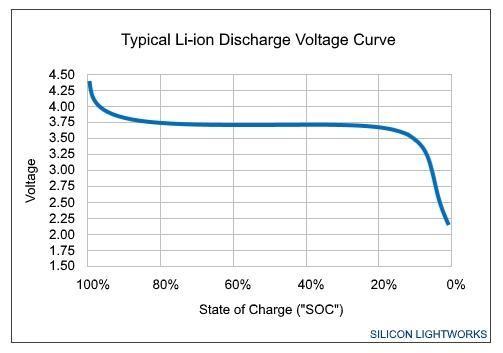
\includegraphics{images/questions/discharge.png}
        \caption{Example of discharge graph of a Li-ion battery}
        \label{fig:discharge}
    \end{figure}
\end{paracol}

% \newpage
\section{Approccio di Kansal}

\begin{figure}[htbp]
   \centering
   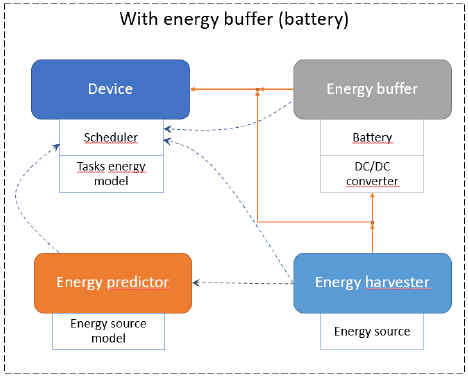
\includegraphics{images/questions/Schermata del 2023-10-20 11-57-01.png}
   % \caption{}
   \label{fig:dom27}
\end{figure}

Il modello di Kansal per la neutralità energetica richiede delle assunzioni sulla fonte energetica, ovvero che sia non controllabile ma prevedibile, o quantomeno che l'\ul{energia da essa prodotta sia approssimabile ad una funzione lineare}.\\
Lo schema in figura è una rivisitazione di quello standard Harvest-Store-Use per implementare Kansal.\\
L'\textit{Energy predictor} realizza una stima della futura produzione di energia suddividendo il tempo in slot di dimensione fissa e usando l'EWMA come modello predittivo; infine comunica i risultati allo \textit{scheduler}.\\
Per ogni possibile duty cycle $dc$ si può calcolare un'utilità $u$ ---che va massimizzata--- e il consumo previsto $c$.
Lo scheduler, in base alle stime fornite dal predictor sull'energia e le informazioni $u$ e $c$ di ciascun $dc$, può assegnare ad ogni slot $dc$, massimizzando $u$ e garantendo la neutralità energetica.\\
Nella pratica questo può tradursi in duty cycle più o meno intensi a seconda dell'energia disponibile.

\subsection{Teorema di Kansal}
Il teorema stabilisce quali sono le condizioni sufficienti (non necessarie) per poter ottenere l'energy neutrality su un sistema.
\begin{align}
    \begin{cases}
        \eta \rho_s \geq \rho_c + \rho_{leak} \quad \text{Trend produzione maggiore di trend consumo e leak} \\
        B_0 \geq \eta \sigma + \delta \quad \text{$B_0$ sufficiente nel worst case} \\
        B_{max} \geq B_0 \quad \text{$B_0$ è un valore legale}
    \end{cases}
\end{align}
\note{Nella seconda equazione ---forse--- $\eta\sigma$ è un termine che starebbe a sinistra con segno negativo, ad indicare che invece di avere una produzione media (compresa fra $+\sigma$ e $-\sigma$) non si produce nulla. $\eta$ = coefficiente di efficienza di carica}

\framedt{Drawback}{
   Uno dei due principali drawback di questo modello è proprio che l'unico parametro che può essere variato per modificare il load è il \textbf{duty cycle}, rendendolo poco adattabile alla gestione di comportamenti più complessi.\\
   Inoltre in caso di sensori, alterare il duty cycle significa avere una misurazione con una \ul{frequenza di \textbf{campionamento} variabile}, che può rendere scomoda l'analisi dei dati.
   }


% Tale approccio prende in considerazione sia l'energia che la carica prevista della batteria, regolando dinamicamente le performance del dispositivo attraverso la regolazione del duty cycle e di conseguenza modificando il carico.

Il modello di Kansal assume che l'energia prodotta si possa approssimare ad una fonte lineare, ovvero che cresce limitata da due rette parallele che hanno un angolo pari a $\rho_s$. Da qui abbiamo che l'energia $E_T$ prodotta in un dato intervallo $[0, T]$ sia uguale a $E_T=\int_0^T P_S(T) dt$ e sia limitata come segue $\rho_s \cdot T-\alpha \leq E_T \leq \rho_s \cdot T+\alpha$ . 

Invece per quanto riguarda il carico (load), il modello di Kansal assume che sia limitato solo superiormente da una retta inclinata di un angolo $\rho_c$ e quindi abbiamo che il carico $L_T$ in un intervallo $[0,T]$ è uguale a $L_T=\int_0^T Pc(T)dt$ e quindi il carico sarà limitato nel seguente modo $0 \leq L_T \leq \rho_c \cdot T+\delta$


\note{
   Nel modello di Kansal il concetto di utility è legato al duty cycle nel seguente modo:
   \ns   
\begin{itemize}
\item $u(dc)=0 $ se $dc < dc_{min}$
\item $u(dc)=\alpha*dc+\beta$ se $dc_{min}\leq dc \leq dc_{max}$
\item $u(dc)=u_M$ se $dc > dc_{max}$
\end{itemize}

Con $u_M$ utility massima, $u_m$ utility minima, $dc_{max}$ duty cycle massimo, $dc_{min}$ duty cycle minimo e con
{\ns
\begin{align}
\alpha=\frac{u_{max}-u_{min}}{dc_{max}-dc_{min}}\\
\beta=u_{min}-\alpha*dc_{min}
\end{align}}
Dove in un grafico con assi $xy$ duty cycle $dc$ e utility $u$, $\alpha$ è il coefficiente lineare (\textit{inclinazione}) della retta, mentre $\beta$ è il punto in cui la retta incrocia l'asse y, ovvero l'\textit{offset} della retta.
}

\subsection{Modello di Kansal}
\begin{itemize}
   \item $k$ il numero di slot in un giorno
   \item $B(i)$ la carica della batteria all'inizio dello slot $i$
   \item $B(k+1)$ la carica della batteria alla fine del giorno
   \item $\tilde{p}_s(i)$ la stima della produzione di energia nello slot $i$
   \item[] \ul{Kansal assegna un $dc(i)$ (dunque una utility $u(i)$) a ciascuno slot $i$ in modo da massimizzare la somma delle utility di tutti gli slot, garantendo che $B(k+1) \geq B(1)$}, ovvero che la carica della batteria alla fine del giorno sia maggiore uguale a quella all'inizio del giorno.
\end{itemize}

\subsection{Algoritmo Kansal}
Si inizializzano gli slot assegnando $dc_{max}$ ai ``sun slot'' e $dc_{min}$ ai ``dark slot''.
A questo punto ---rispetto alla stima di produzione di energia $\tilde{p}_s(i)$--- si può riscontrare:
\begin{enumerate}
   \item \textbf{Overproduction}\\
   Si massimizza il $dc$ dei dark slot finché non si esaurisce l'energia sovrapprodotta
   \item \textbf{Underproduction}\\
   Si minimizza il $dc$ dei sun slot finché non si va in pari con l'energia prodotta
\end{enumerate}
\section{Modello basato su task}

\begin{figure}[htbp]
   \centering
   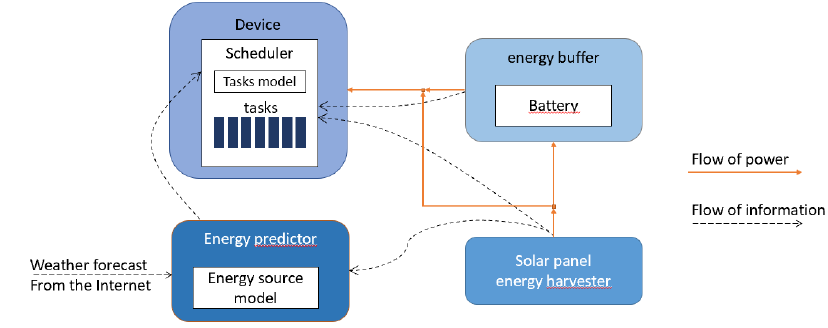
\includegraphics{images/questions/Schermata del 2023-10-20 11-57-15.png}
   % \caption{}
   \label{fig:dom28}
\end{figure}

{\ns Il task-based model si basa sull'idea che il ciclo di funzionamento di un applicazione di un dispositivo IoT sia tipicamente:
\begin{enumerate}
   \item \textbf{Sensing}
   \item \textbf{Storing}
   \item \textbf{Processing}
   \item \textbf{Transmitting}
\end{enumerate}
Ciascuna di queste fasi può avere più implementazioni possibili con consumi energetici potenzialmente diversi.
Ad esempio, potrebbero essere disponibili sensori diversi, sampling rate variabili\dots Si potrebbe fare processing e storing solo di alcuni dati, o di trasmettere dati compressi o meno, già processati o da processare, cifrati o in chiaro, ecc\dots}
Dunque è possibile definire l'implementazione di un'applicazione IoT come un insieme di \textbf{task}, ciascuna con un consumo energetico per unità di tempo e un'utilità.
\note{Il numero di task è limitato dai vincoli del dispositivo e dallo scheduling ma le funzioni generali non cambiano, cambia l'implementazione che ha effetto sul comportamento del dispositivo.}

Similmente a come accade per Kansal, sulla base della stima di produzione di energia e del consumo di ciascun task, uno scheduler assegna un task per ciascuno slot di tempo,
risolvendo un problema di ottimizzazione NP-Hard attraverso una soluzione (leggermente approssimativa) pseudo-polinomiale basata su programmazione dinamica.

Il vantaggio rispetto a Kansal è che al posto di duty cycle diversi, si assegnano task, permettendo un più agevole e modulare adattamento del carico di lavoro.  

\section{Diffusione diretta}

\begin{figure}[htbp]
   \centering
   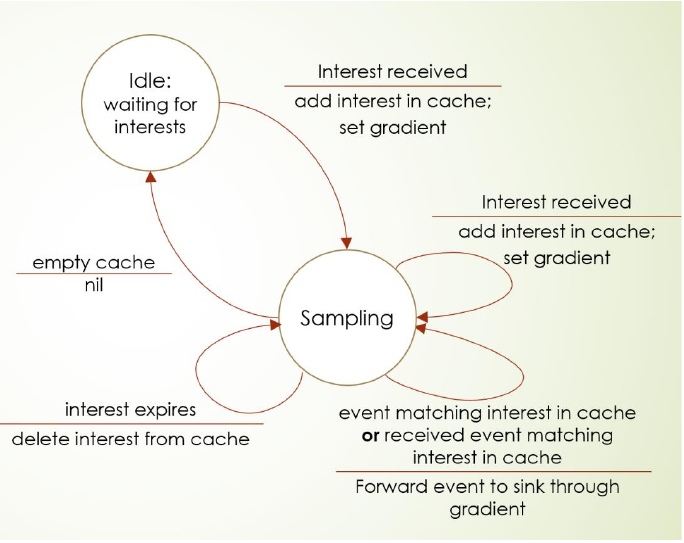
\includegraphics{images/questions/Schermata del 2023-10-20 12-12-43.png}
   % \caption{}
   \label{fig:dom29}
\end{figure}

Protocollo di rete per WSN che specifica come eseguire sensing distribuito e rispondere a query basate sul contenuto dei dati, i quali sono associati a coppie \textbf{attributo-valore}.
Può essere diviso in 3 passi:

\begin{enumerate}
\item \emph{Comunicazione basata sull'interesse}: la comunicazione si basa sull'interesse espresso dai sink node (nodi che fungono da output gateway verso reti esterne) verso tipi di dati o attributi, il quale propaga la query nella rete;
\item \emph{Propagazione dei dati basata su gradiente}: ricevute le query dai sink i sensori iniziano a raccogliere i dati al più ampio sampling rate fra quelli dei gradienti locali.
\note{Un \textbf{gradiente} esprime una \textit{direzione} (verso il sink richiedente) e un data rate.}
I nodi inoltrano i dati verso i sink node solo se hanno in cache l'interesse (con relativo gradiente) che matcha il dato e se il dato non è già stato inoltrato prima.
\item \emph{Aggregazione e Reinforcement}: mentre i dati confluiscono verso il sink node, i nodi sensore intermedi mettono in cache gli interessi ricevuti (fino all'expire time) e aggregano i dati relativi a uno stesso interesse con sampling rate differenti.\\
Il sink può ricevere dati da più sorgenti, e per evitare ciò, può scegliere di fare \textit{Reinforcement} su uno dei path (quello che il maggiore data rate) e inviarvi un interest con data rate maggiore, che verrà propagato lungo quel path.
In questo modo vengono empiricamente (\textred{?}) preferiti i dati di migliore qualità.
% \item \emph{Adattamento basato sul feedback}: i sink node forniscono un feedback ai sensori rinforzando o sopprimendo i flussi di dati. Questo aiuta ad ottimizzare i percorsi di routing e migliora l'efficienza energetica nella rete.
\end{enumerate}

Nell'immagine si vede la macchina a stati di un sensore, partendo dall'\texttt{idle} state, in cui il dispositivo è in attesa di un interest.
Quando viene ricevuto un interest questo viene aggiunto alla cache, viene impostato il gradiente avente come direzione il nodo da cui proviene il messaggio di interest e come data rate quello specificato nell'interest (campo \texttt{interval}); il nodo passa allo stato di \texttt{sampling}, se non vi è già.\\
Quando il sensore rileva un evento associato con un interesse in cache (e.g. ``sta passando un elefante''), inizia il campionamento dell'evento e vengono inviati al sink node in accordo con il gradiente registrato per quell'interest.\\
A ciascun interest è associata una \texttt{duration}, al termine della quale l'interest viene rimosso dalla cache, che quando vuota porta allo stato \texttt{idle}.\\
La macchina a stati è implementata su interruzioni ---similmente a TinyOS--- permettendo a un dispositivo di agire contemporaneamente come router e come sensore.

\section{GPSR Modalità Greedy forwarding}

\begin{figure}[htbp]
   \centering
   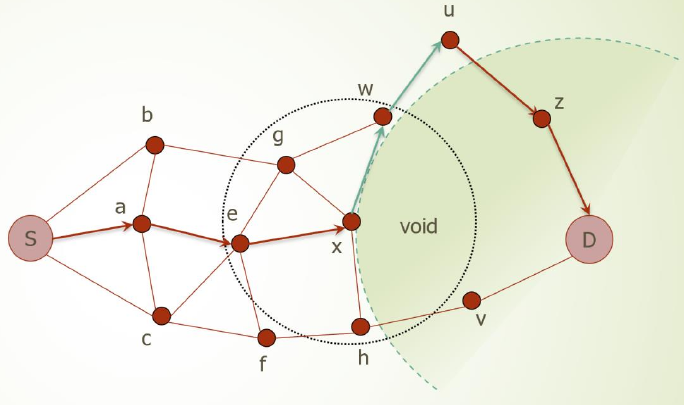
\includegraphics{images/questions/Schermata del 2023-10-20 12-13-24.png}
   % \caption{}
   \label{fig:dom30}
\end{figure}

La DD richiede alcune assunzioni:
\begin{itemize}
   \item Un \ul{singolo} nodo Sink con $id = 0$ \ul{permanentemente connesso} alla rete (se va down la rete non funziona più)
   \note{\textred{In realtà forse potrebbero esserci più sink}}
   \item Ogni nodo con \ul{$id$ univoco}
   \item Il sink inizializza e mantiene il routing tree
   \item I messaggi dei nodi sono unicast diretti verso il sink
   \item Solo il sink può mandare messaggi broadcast
\end{itemize}
Notare che la DD non sfrutta le capacità di processing dei nodi e non permette neanche il rilevamento di eventi ``compositi'' distribuiti su più sensori.
La Directed Diffusion non è scalabile per reti grandi e porta a colli di bottiglia in prossimità dei sink con topologie ad albero. Topologie diverse richiedono strategie di routing diverse, e per questo motivo è stato proposto il protocollo GPSR.

Greedy Perimeter Stateless Routing (o GPRS) è un protocollo alternativo al protocollo Direct Diffusion che permette il routing dei pacchetti nodo-a-nodo senza mantenere uno stato globale e con un basso overhead. 
Anche questo protocollo necessita alcune assunzioni, ma meno stringenti:

\begin{itemize}
\item i nodi sono disposti in uno spazio bidimensionale;
\item i nodi conoscono la posizione geografica dei loro vicini;
\item il nodo sorgente S conosce la posizione geografica del nodo destinazione D.
\end{itemize}

GPRS può operare sotto due modalità diverse, \textbf{\emph{greedy forwarding}} e \textbf{\emph{perimeter mode}}.

Inizialmente si applica il \textit{greedy forwarding}: la sorgente S per inviare un pacchetto alla destinazione D inoltra il pacchetto al nodo neighbour geograficamente più vicino alla destinazione.\\
Questa modalità ``fallisce'' quando si entra in una regione di vuoto, i.e. non ci sono nodi che più vicini a D;
Quando ciò si verifica avviene lo switch in \textit{perimeter mode} che identifica il perimetro della regione vuota e lo percorre (seguendo LHL o RHR rule) fino a trovare un nodo che possiede un vicino geograficamente \ul{più vicino alla destinazione rispetto al nodo che ha fatto lo switch in perimeter mode}\footnote{Non può avvenire appena si esce dalla void region, in quanto ciò potrebbe portare a loop}, momento in cui torna alla \textit{greedy mode} per raggiungere la destinazione.



\note{Nell'immagine su x si passa in perimeter mode, fino ad arrivare a u, che ha come vicino z che è geograficamente più vicino a D rispetto ad x.}

\section{GPSR Modalità Perimeter forwarding}

\begin{figure}[htbp]
   \centering
   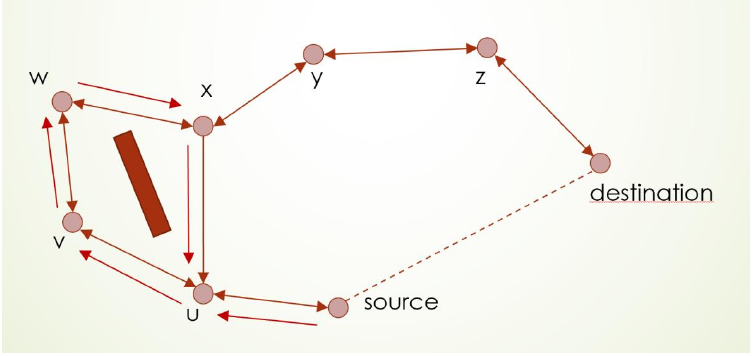
\includegraphics{images/questions/Schermata del 2023-10-20 12-13-49.png}
   % \caption{}
   \label{fig:dom31}
\end{figure}

In questo caso c'è un ostacolo che può portare a un loop.
\begin{enumerate}
   \item Nel nodo sorgente avviene subito lo switch alla perimeter mode.
   \item l'arco $(x,u)$ è unidirezionale, dunque u inoltra il pacchetto a v.
   \item $v$ non vede $x$, e dunque inoltra il pacchetto a $w$.
   \item $w$ inoltra il pacchetto a $x$.
   \item $x$ se utilizza \texttt{RHR}, \ul{il primo arco che trova in senso antiorario partendo da $(w,x)$ è $(x,u)$}, e dunque inoltra il pacchetto a $u$, \ul{portando a un \textbf{loop}}.\\
   Se invece si utilizza \texttt{LHL}, gli step precedenti non cambiano, ma $x$ inoltrerà il pacchetto a $y$, dove si passerà alla greedy mode e si giungerà alla destinazione.
\end{enumerate}

\textit{Mutual Witness}, estensione di planarization algorithm può risolvere questo problema usando sempre link bidirezionali; tuttavia, ci sono casi in cui l'aggiunta di tali link bidirezionali porta a grafi non planari e a loop, rendendolo non idoneo per scenari reali.

\section{GPSR Planarizzazione del grafo}

\begin{figure}[htbp]
   \centering
   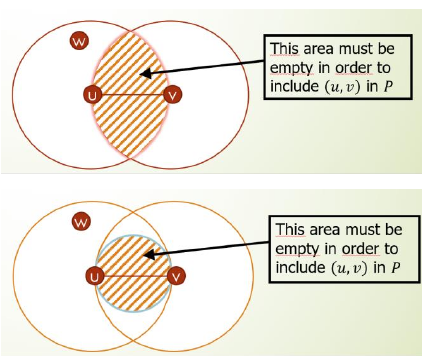
\includegraphics{images/questions/Schermata del 2023-10-20 12-14-06.png}
   % \caption{}
   \label{fig:dom32}
\end{figure}

Il grafo della topologia di rete tipicamente non è \textit{planare} (i.e. gli archi potrebbero incrociarsi), per questo motivo è necessario costruire una rappresentazione del grafo che lo sia.
{\ns Abbiamo discusso due metodi:
\begin{itemize}
\item \textbf{Relative neighborhood Graph of G (RNG)}
does not exist a third point $w$ that is closer to both $u$ and $v$ than they are to each other
\[
(u,v) \in P \Leftrightarrow (u,v) \in G \wedge d(u,v) \leq \max_{\forall w\in N(u)\cup N(v)} (d(u,w),d(v,w))
\]
\note{Considerati tutti i vicini di u e v, non esiste un nodo w la cui distanza sia da v che da u sia minore di d(u,v), cioè la distanza fra u e v stessi}
\item \textbf{Gabriel Graph (GG)}\\
Questa opzione porta a un grafo planarizzato più denso.\\
La legge matematica per costruirlo è \st{simile a Pitagora \smiley} :
\[
(u,v) \in P \Leftrightarrow (u,v) \in G \wedge d(u,v)^2 \leq d(u,w)^2 + d(v,w)^2 \quad \forall w \in N(u) \cup N(v)
\]
\note{Considerati tutti i vicini di u e v, non esiste un nodo w la cui somma dei quadrati delle distanze fra u e v sia minore del quadrato della distanza d(u,v). In altre parole, preso il triangolo u,v,w, il quadrato del lato fra u,v è minore della somma fra gli altri due}
\end{itemize}}
Entrambi gli algoritmi creano un sottografo $P$ a partire da un grafo $G$ dato, senza aggiungere archi, ma solo rimuovendoli. 
\note{Alcune proprietà vengono mantenute: ad esempio, se un grafo è connesso allora anche il suo sottografo sarà connesso.}

\note{Inoltre, entrambi gli algoritmi minimizzano l'overhead di memoria e di calcolo eseguendo una knowledge discovery distribuita e localizzata per identificare gli archi del grafo planarizzato. Questo è reso possibile perché ogni nodo ha eseguito la planarizzazione del grafo in anticipo.}